\begin{frame}{Solución}
    \begin{columns}
        \column{.5\textwidth}
        Antes de que un computador se dañe:
        \begin{itemize}
            \item Reconocer los procesos
            \item Mesurar las capacidades del computador
            \item Retirar los elementos innecesarios
            \item Identificar alternativas \parencite{free}
        \end{itemize} \pause
        \column{.5\textwidth}
        Después de que el mismo quede defectuoso:
        \begin{itemize}
            \item Saber lo que uno necesita
            \item Reconocer los costes
            \item Identificar las ventajas y desventajas en la
            compra
        \end{itemize}
        No únicamente para los programadores como afirma \parencite{trejos}
    \end{columns}
\end{frame}
\begin{frame}{Solución}
    \framesubtitle{Desarrollo}
    \begin{itemize}
        \item Un esquema frecuente para el desarrollo de software 
        \parencite{devops}
        \item Compilación 
        \item Un medio para simular el software
        \item Realizar la optimización \textcite{rodriguez} para dar
        los buenos resultados
    \end{itemize}
\end{frame}
\begin{frame}{Solución}
    \framesubtitle{gnome-system-monitor}
    \begin{center}
        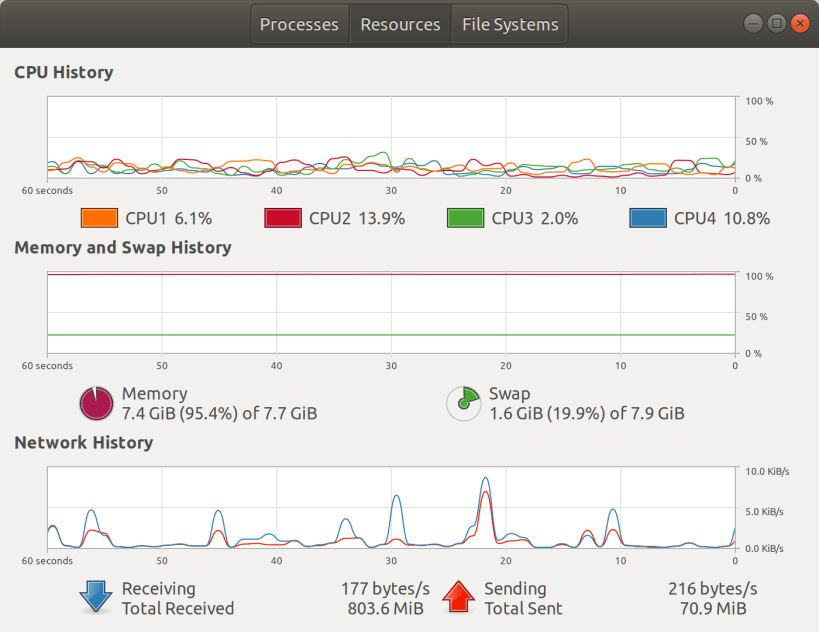
\includegraphics[height=.6\textheight]{./pictures/gsm.png} \\
        Un gestor de procesos para Gnome, de libre acceso y
        sumamente intuitivo
    \end{center}
\end{frame}
\begin{frame}{Solución}
    \framesubtitle{LAN}
    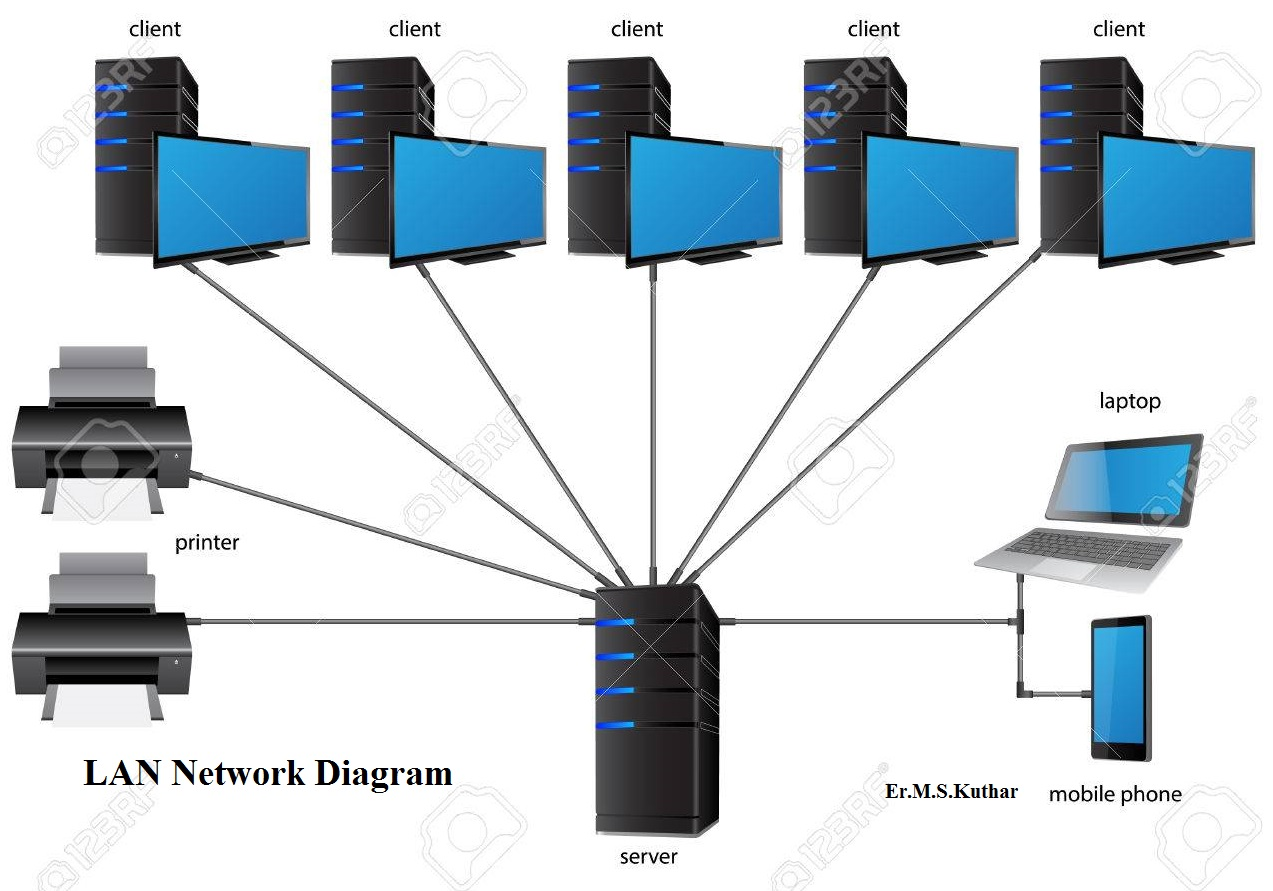
\includegraphics[height=0.75\textheight]{./pictures/lan.jpg}
\end{frame}
\begin{frame}{Solución}
    \framesubtitle{Requerimientos}
    \begin{itemize}
        \item Notificar al usuario cuando haya una anomalía
        \item Contener las funcionalidades básicas teniendo como
        base un software de ITAM
        \parencite{invgate}
        \begin{itemize}
            \item Analizar software
            \item Ser capaz de analizar las partes del computador
            a nivel de hardware
            \item Aconsejar las mejores opciones de acuerdo a sus
            analisis
        \end{itemize}
        \item Contener una guía para el usuario
        \item Utilidad en una LAN (Local Area Network)
        \parencite{invgate}
        \item De "libre" acceso \parencite{free}
    \end{itemize}
\end{frame}